\documentclass[titlepage]{article}

\usepackage[utf8]{inputenc}
\usepackage[T1]{fontenc}
\usepackage[french]{babel}
\usepackage{mathtools, amssymb, amsthm, amsmath}
\usepackage{lmodern}
\usepackage{color}
\usepackage[table]{xcolor}
\usepackage{listings}
\usepackage{hyperref}
\usepackage{geometry}

\title{\Huge{La réussite des alliances}}
\author{\Large{Florian Berger - Lucas Lesage}\\ \Large{Binôme 5}}
\date{Printemps 2022}

\definecolor{darkWhite}{rgb}{0.94,0.94,0.94}

\geometry{hmargin=2.5cm,vmargin=2.5cm}
\parskip=5pt

\lstset{language=python,
		backgroundcolor=\color{darkWhite},  		
  		breakatwhitespace=false,
		breaklines=true,
  		commentstyle=\color{red},
  		escapeinside={\%*}{*)},
  		rulecolor=\color{black},
  		showstringspaces=false,
  		stringstyle=\color{gray},
  		frame=tb, 
  		xleftmargin=-5pt,
  		xrightmargin=0pt,
  		tabsize=4}


\begin{document}
\maketitle

\tableofcontents


\newpage
\section*{Avant-propos}
\addcontentsline{toc}{section}{Avant-propos}

Le projet présenté dans ce document est la réalisation d’un programme en Python permettant de jouer à une forme de réussite nommée « réussite des alliances », aussi appelée « la poussette ». 

\subsection*{Règles du jeu}
\addcontentsline{toc}{subsection}{Règles du jeu}
\hypertarget{avant-propos}{Cette réussite} peut être jouée avec un jeu de 32 ou de 52 cartes. \par
La partie commence en alignant trois cartes, de gauche à droite. On observe ensuite la carte située en avant-dernière position. \vspace{5pt}
	\begin{itemize}
	\item[$\bullet$] Si elle est entourée de cartes ayant la même valeur ou la même couleur (on appellera une telle configuration une « alliance »), on prend la carte située au milieu et on la met sur la carte située immédiatement à sa gauche (on parle de « saut ») ;
	\item[$\bullet$] Sinon, on pioche une nouvelle carte, que l’on pose à droite de la dernière carte.
	\end{itemize}\par
\vspace{5pt}Une fois la carte posée, on observe l’avant-dernière carte, et on reproduit le schéma décrit ci-dessus.\par  
Si un saut a pu être fait, on vérifie si d’autres alliances apparaissent. On peut alors effectuer les différents sauts possibles, consécutivement.
La partie se termine une fois que la dernière carte de la pioche est posée et qu’aucun saut n’est possible.\par 
Traditionnellement, la partie est gagnée lorsqu’il ne reste plus que deux tas de cartes, condition assez difficile à atteindre, et plus particulièrement avec un paquet de 52 cartes.\par 

\subsection*{Réalisation du projet}
\addcontentsline{toc}{subsection}{Réalisation du projet}

Ce projet a été réalisé tout au long du second semestre de l'année universitaire 2021-2022. Le premier cours nous a permis d'identifier les caractéristiques principales du projet, et d'établir quelles extensions nous souhaitions réaliser.\par
Chaque séance débutait par un récapitulatif de nos avancées respectives sur le programme. Nous présentions les fonctions que nous avions réalisées, et discutions des éventuelles modifications à apporter. A ce titre, bien que le concepteur de chaque fonction sera indiqué à la suite de ce document, il est important de tenir compte du fait qu'elles ont été sujettes à discussions et ont été améliorées collectivement.\par


\subsection*{Lien vers le projet}
\addcontentsline{toc}{subsection}{Lien vers le projet}

\url{https://gitlab.isima.fr/lulesage/jeu-de-la-reussite-par-florien-berger-et-lucas-lesage.git}

\newpage
\section{Fonctions de formatage}
\label{sec : format}

\noindent	\begin{minipage}{\textwidth}
	\begin{lstlisting}
	cree_carte(couleur, valeur)	
	\end{lstlisting}
	\end{minipage}
	
\emph{\textbf{conçue par : } Florian Berger} \vspace{2mm}\par
La fonction prend en argument un caractère \textbf{couleur} et un caractère ou un entier \textbf{valeur}, et renvoie une carte au format dictionnaire.\vspace{1mm}\par
\underline{Exemple} : \texttt{cree\_carte('K', 10)} renvoie \texttt{\{'valeur':10, 'couleur':'K'\}}\par
\vspace{5mm}

\label{fun : carte_to_chaine}
\noindent	\begin{minipage}{\textwidth}
	\begin{lstlisting}
	carte_to_chaine(carte, char_special = True)
	\end{lstlisting}
	\end{minipage}
	
\emph{\textbf{conçue par : } Lucas Lesage} \vspace{2mm}\par

La fonction prend en argument une carte ainsi qu’un booléen char\_special. La fonction renvoie une carte au format string. Cependant, en fonction de la valeur de char\_special cela peut être soit avec les symboles des couleurs des cartes ou au format valeur-couleur.\vspace{1mm}\par
\underline{Exemple} : \texttt{carte\_to\_chaine(\{'valeur': 9, 'couleur': 'K'\})} renvoie 9$\diamondsuit$ et \texttt{carte\_to\_chaine(\{'valeur': 9, 'couleur': 'K'\}, False)} renvoie 9-K \par
\vspace{5mm}
	
\noindent	\begin{minipage}{\textwidth}
	\begin{lstlisting}
	chaine_to_dico(carte)
	\end{lstlisting}
	\end{minipage}
	
\emph{\textbf{conçue par : } Florian Berger} \vspace{2mm}\par
La fonction prend en argument une chaine de caractère \textbf{carte} au format \texttt{"valeur-couleur"}, et renvoie un dictionnaire désignant une carte au format \texttt{\{'valeur': valeur, 'couleur': couleur\}}.\par
Si la valeur de la carte est un entier, la valeur contenue dans le dictionnaire retourné est un entier. S'il s'agit d'une lettre \texttt{'A', 'R', 'D'} ou \texttt{'V'}, la valeur contenue dans le dictionnaire sera un caractère.\vspace{1mm}\par
\underline{Exemples} : \texttt{chaine\_to\_dico('9-T')} renvoie \texttt{\{'valeur':9, 'couleur':'T'\}}\par
\hspace*{1.75cm}\texttt{chaine\_to\_dico('R-T')} renvoie \texttt{\{'valeur':'R', 'couleur':'T'\}}\par
\vspace{5mm}

\noindent	\begin{minipage}{\textwidth}
	\begin{lstlisting}
	paquet_to_liste_dico(paquet)
	\end{lstlisting}
	\end{minipage}
	
\emph{\textbf{conçue par : } Florian Berger} \vspace{2mm}\par
La fonction prend en argument une liste de chaines de caractères \textbf{paquet} au format \texttt{['valeur1-couleur1', 'valeur2-couleur2',...]}, et renvoie une liste de dictionnaires au format \texttt{[\{'valeur': valeur1, 'couleur': couleur1\}, \{'valeur': valeur2, 'couleur': couleur2\},...]}.\vspace{1mm}\par
\underline{Exemple} :\par
\texttt{paquet\_to\_liste\_dico(['5-K', 'D-P'])} renvoie \texttt{[\{'valeur':5, 'couleur':'K'\}, \{'valeur':'D', 'couleur':'P'\}]}\par
\vspace{5mm}
	
\noindent	\begin{minipage}{\textwidth}
	\begin{lstlisting}
	cree_paquet_cartes(nb_cartes)
	\end{lstlisting}	
	\end{minipage}

\emph{\textbf{conçue par : } Florian Berger et Lucas Lesage} \vspace{2mm}\par
La fonction prend en argument un entier \textbf{nb\_cartes} et renvoie une liste de chaines de caractères appelée paquet au format \texttt{['valeur1-couleur1', 'valeur2-couleur2',...]}. \par
Un paquet compte 32 ou 52 cartes selon l'entier mis en argument, rangées par couleur puis par valeur. Si l'entier mis en argument est différent de 32 ou 52, le paquet renvoyé est vide.\par

\bigskip

Ces différentes fonctions dites "de formatage" ont pour but, comme leur nom l'indique, de changer le type associé à une carte ou à un paquet de cartes afin de pouvoir les exploiter dans d'autres fonctions décrites ultérieurement.\par
A titre d'exemple, la fonction \texttt{paquet\_to\_liste\_dico} permettra de formater une pioche conservée dans un fichier de sauvegarde au format chaine de caractères en liste de dictionnaires, afin qu'elle soit utilisable dans un mode de jeu.

\newpage \section{Fonctions principales}
\label{sec : principal}

\noindent	\begin{minipage}{\textwidth}
	\begin{lstlisting}
	init_pioche_alea(nb_carte = 32)
	\end{lstlisting}	
	\end{minipage}

\emph{\textbf{conçue par : } Lucas Lesage} \vspace{2mm}\par
La fonction prend en argument un entier nb\_carte, et renvoie un paquet de carte mélangé. \vspace{1mm}\par
L’objectif de la fonction init pioche alea est de prendre un paquet de carte est de le mélanger. Pour cela, nous avons utilisé la fonction shuffle de la bibliothèque random. \vspace{5mm}

\noindent	\begin{minipage}{\textwidth}
	\begin{lstlisting}
	afficher_reussite(liste_carte)
	\end{lstlisting}	
	\end{minipage}

\emph{\textbf{conçue par : } Florian Berger} \vspace{2mm}\par
La fonction prend en argument une liste de cartes \textbf{liste\_carte}, au format liste de dictionnaires, et affiche chaque carte de cette liste au format \texttt{'Valeur Symbole'} au moyen de la fonction \texttt{carte\_to\_chaine} (voir section \ref{fun : carte_to_chaine}).\par
\vspace{5mm}
	
\noindent	\begin{minipage}{\textwidth}
	\begin{lstlisting}
	alliance(carte1, carte2)
	\end{lstlisting}	
	\end{minipage}

\emph{\textbf{conçue par : } Florian Berger} \vspace{2mm}\par
La fonction prend en argument deux cartes au format dictionnaire,  \textbf{carte1} et \textbf{carte2}, et renvoie :
\begin{itemize}
\item Vrai si elles ont la même \texttt{'valeur'} ou la même \texttt{'couleur'} ;
\item Faux sinon.
\end{itemize}
\par
\vspace{5mm}

\label{fun : saut_si_possible}
\noindent	\begin{minipage}{\textwidth}
	\begin{lstlisting}
	saut_si_possible(liste_tas, num_tas)
	\end{lstlisting}	
	\end{minipage}

\emph{\textbf{conçue par : } Florian Berger} \vspace{2mm}\par
La fonction prend en arguments :
	\begin{itemize}
	\item une liste de cartes \textbf{liste\_tas}, au format liste de dictionnaires, qui représente les cartes révélées au joueur, 
	\item un entier \textbf{num\_tas}, représentant l'indice de la carte pour laquelle on veut vérifier la possibilité de faire un saut,
	\end{itemize}
\par 
et renvoie :
	\begin{itemize}
	\item Vrai si le saut est possible ;
	\item Faux sinon.
	\end{itemize}
\par
La fonction vérifie également si l'entier \textbf{num\_tas} correspond à un indice inclus dans la liste de tas et permettant un saut, c'est-à-dire s'il est compris entre la deuxième carte (qui aura pour indice 1) et l'avant-dernière carte de la liste. Dans le cas contraire, la fonction renverra Faux.
\vspace{5mm}

\label{fun : une_etape_reussite}
\noindent	\begin{minipage}{\textwidth}
	\begin{lstlisting}
	une_etape_reussite(liste_tas, pioche, affiche = False)
	\end{lstlisting}	
	\end{minipage}

\emph{\textbf{conçue par : } Florian Berger} \vspace{2mm}\par
La fonction prend en arguments :
	\begin{itemize}
	\item une liste de dictionnaires \textbf{liste\_tas}, correspondant aux cartes révélées face au joueur,
	\item une liste de dictionnaires \textbf{pioche}, correspondant aux cartes restant dans la pioche,
	\item un booléen \textbf{affiche}, en argument optionnel, initialisé par défaut à Faux,
	\end{itemize}
	\par
et réalise une étape de la réussite selon le schéma suivant :
	\begin{enumerate}
	\item On pioche une carte et on l'ajoute à la liste des tas en jeu,
	\item On vérifie la possibilité de réaliser un saut à l'avant-dernière carte de la liste au moyen de la fonction \texttt{saut\_si\_possible} :
		\begin{itemize}
		\item[$\bullet$] Si oui :
			\begin{itemize}
			\item[$\rightarrow$] On réalise le saut, 
			\item[$\rightarrow$] On se place à la deuxième carte de la liste en partant de la gauche, 
			\item[$\rightarrow$] On vérifie si un saut est possible, et on le réalise tant que cela est possible à cet emplacement,
			\item[$\rightarrow$] Une fois qu'on ne peut plus faire de saut à cet emplacement, on passe au tas situé immédiatement à droite, et on renouvelle la vérification à partir de ce tas,
			\item[$\rightarrow$] On réalise cette étape jusqu'à arriver à la dernière carte de la liste ;
			 \end{itemize}
		\item[$\bullet$] Si non, la fonction s'arrête.
		\end{itemize}
	\end{enumerate}
\par
Si l'argument \textbf{affiche} est initialisé à Vrai, alors la fonction affichera, au moyen de la fonction \texttt{afficher\_reussite}, la liste de tas en jeu à chaque modification de cette liste, c'est-à-dire à l'étape de pioche et à chaque saut réalisé.\par
Afin de ne manquer aucune possibilité de saut, nous avons convenu de recommencer la vérification d'existence d'alliances à partir de la deuxième carte de la liste à chaque fois qu'un saut est effectué. En effet, il arrive que la réalisation d'un saut entraine l'apparition d'alliances à des emplacements d'indice inférieur à celui en cours de vérification. 

\newpage \section{Modes de jeu}
\label{sec : modes_jeu}

\noindent	\begin{minipage}{\textwidth}
	\begin{lstlisting}
	reussite_mode_auto(pioche, affiche = False)
	\end{lstlisting}	
	\end{minipage}

\emph{\textbf{conçue par : } Florian Berger} \vspace{2mm}\par
La fonction prend en argument une liste de cartes \textbf{pioche}, au format liste de dictionnaires, et en argument optionnel un booléen \textbf{affiche}, initialisé à Faux par défaut. Elle réalise les différentes étapes d'une partie de réussite des alliances selon les règles décrites dans la rubrique \hyperlink{avant-propos}{"Avant-propos"}.
	\begin{itemize}
	\item Tant que la pioche n'est pas vide, elle utilise la fonction \texttt{une\_etape\_reussite} (voir section \ref{fun : une_etape_reussite}) à chaque nouvelle carte piochée.
	\item Une fois la pioche vide, il convient de vérifier s'il reste des sauts possibles. Pour ce faire, on applique à chaque carte à partir de la deuxième carte à gauche la fonction \texttt{saut\_si\_possible} (voir la section \ref{fun : saut_si_possible}), autant de fois qu'un saut est possible, puis on passe au tas suivant, jusqu'à atteindre le dernier tas de la liste.
	\end{itemize}\par
Si l'argument \textbf{affiche} est initialisé à Vrai, la fonction affichera, au moyen de la fonction \texttt{afficher\_reussite} :
	\begin{itemize}
	\item La pioche utilisée pour jouer la partie,
	\item La liste de tas en jeu à chaque modification de cette liste, c'est-à-dire à chaque pioche et à chaque saut réalisé.
	\end{itemize}
\par
Elle renvoie une liste de dictionnaires représentant les cartes visibles une fois la partie terminée.
\vspace{5mm}

\noindent	\begin{minipage}{\textwidth}
	\begin{lstlisting}
	reussite_mode_manuel(pioche, nb_tas_max = 2)
	\end{lstlisting}	
	\end{minipage}

\emph{\textbf{conçue par : } Florian Berger} \vspace{2mm}\par
La fonction prend en argument une liste de cartes \textbf{pioche}, au format liste de dictionnaires, et en argument optionnel un entier \textbf{nb\_tas\_max}, initialisé à 2 par défaut, qui représente le nombre de tas à ne pas dépasser en fin de partie pour déclarer que l'utilisateur a gagné.\par
Elle permet à l'utilisateur de simuler une partie de réussite des alliances. A chaque étape, un menu s'affiche et propose plusieurs options :
	\begin{enumerate}
	\item Piocher une carte, tant que la pioche n'est pas vide. Dans le cas contraire, cette option n'est plus affichée ;
	\item Proposer un saut : l'utilisateur sera alors invité à saisir l'indice de la carte sur laquelle il souhaite réaliser le saut. Si le saut est possible, il est effectué. Sinon, un message d'erreur apparaît, suivi du menu du mode manuel. Si l'indice saisi n'est pas valide, l'utilisateur est invité à saisir un nouvel indice ;
	\item Quitter : dans ce cas, les cartes sont tirées consécutivement, sans vérifier si un saut est possible, jusqu'à ce que la pioche soit vide.
	\end{enumerate}\par

Une fois la partie terminée, si le nombre de tas restant est inférieur à l'entier \textbf{nb\_tas\_max}, un message \texttt{"Reussite !"} apparaît. Sinon, le message affiché sera \texttt{"Perdu..."}.\par
La conception de cette fonction n'a pas été sans difficultés. La première a été la conception d'un menu permettant au joueur d'effectuer les actions de son choix. L'implémentation d'une boucle \texttt{while} prenant en compte une valeur \textbf{reponse} saisie par l'utilisateur nous a semblé être une bonne solution, qui a cependant nécessité de réaffecter une valeur neutre à la variable \textbf{reponse} (ici, 0) dans les cas où le joueur décide d'effectuer une pioche ou de proposer un saut. Cette réaffectation permet d'afficher à nouveau le menu de jeu tant que la partie est en cours.\par
La seconde difficulté a été la gestion de la partie une fois la pioche vide. En effet, dans sa première version, la fonction ne proposait pas d'effectuer de saut une fois la dernière carte tirée, ce qui empêchait automatiquement d'atteindre les conditions de victoire si le nombre de tas maximal était fixé à 2. Il a fallu donc prévoir la situation où la pioche est vide et où le joueur n'a pas choisi de quitter la partie en cours. Un nouveau menu, permettant uniquement de proposer un saut ou de quitter, a été mis en place sur le même principe que le précédent.

\vspace{5mm}

\noindent	\begin{minipage}{\textwidth}
	\begin{lstlisting}
	lance_reussite(mode, nb_carte = 32, affiche = False, nb_tas_max = 2)
	\end{lstlisting}	
	\end{minipage}

\emph{\textbf{conçue par : } Lucas Lesage} \vspace{2mm}\par

La fonction prend en argument une chaine de caractère mode (définissant le mode de jeu), un entier nombre de carte, un booléen affiche et un entier nb\_tas\_max. Et qui lance une partie choisie par le mode de jeu désiré. \vspace{1mm}\par
L’objectif la fonction est de pouvoir lancer une partie en mode automatique ou en mode manuel.\vspace{5mm}

\newpage \section{Chargement / sauvegarde de partie}
\label{sec : charg-sauv}
\noindent	\begin{minipage}{\textwidth}
	\begin{lstlisting}
	init_pioche_fichier(nom_fichier)
	\end{lstlisting}	
	\end{minipage}

\emph{\textbf{conçue par : } Lucas Lesage} \vspace{2mm}\par

La fonction prend en argument une chaine de caractère nom\_fichier. Et qui renvoie une liste de carte qui aura été lue dans un fichier. \vspace{5mm}

\noindent	\begin{minipage}{\textwidth}
	\begin{lstlisting}
	ecrire_fichier_reussite(nom_fichier_sauvegarde, pioche)
	\end{lstlisting}	
	\end{minipage}

\emph{\textbf{conçue par : } Lucas Lesage} \vspace{2mm}\par

 La fonction prend en argument une chaine de caractère nom\_fichier ainsi qu’une liste pioche. La fonction ne renvoie rien mais écris dans un fichier les cartes composant la pioche.
 
 \vspace{5mm}
 
L’objectif de ces fonctions est de pouvoir lire et sauvegarder des parties à partir d’un fichier. Nous avons pu observer une difficulté au niveau de la fonction écrire réussite sur le point de vue du format approprié à inscrire. 
Pour la fonction init pioche fichier, nous avons tout d’abord transformé, le fichier en une liste de carte au format valeur-couleur (10-P). Puis nous avons transformée chacune des cartes au format de dictionnaire de carte (ex : \{‘valeur’ : 10, ‘couleur’ : ’P’\}) grâce à la fonction chaine to dico. 
Pour la fonction écrire fichier, nous avons décidé de parcourir la liste de carte au format dictionnaire pour les transformer en des cartes au format valeur-couleur au moyen de la fonction carte to chaine puis de les écrire dans le fichier désiré.

\vspace{5mm}


\newpage \section{Menu du jeu}
\label{sec : menu}
\noindent	\begin{minipage}{\textwidth}
	\begin{lstlisting}
	menu_reussite()
	\end{lstlisting}	
	\end{minipage}

\emph{\textbf{conçue par : } Florian Berger} \vspace{2mm}\par
La fonction ne prend aucun argument, et constitue l'unique fonction de notre programme principal. Elle permet à l'utilisateur d'effectuer les fonctionnalités suivantes :
	\begin{itemize}
	\item Jouer une partie ;
	\item Effectuer une simulation ;
	\item Quitter le programme.
	\end{itemize}
	\par

Nous avons décidé de concevoir cette fonction suite à un constat simple : dans le cadre de la réalisation de ce projet, il nous a été proposé de mettre en place les fonctions \texttt{init\_pioche\_fichier} et \texttt{ecrire\_fichier\_reussite}, qui permettent la mise en place d'un système de chargement / sauvegarde de pioche (pour plus de précisions, voir la section \ref{sec : charg-sauv}). Cependant, celles-ci ne sont pas utilisées dans le cadre des consignes proposées. Nous avons donc réfléchi à la meilleure façon de les intégrer au jeu, tout en conservant l'accessibilité du programme.\par
Nous avons donc conçu une fonction réunissant la majorité des fonctionnalités prévues dans le programme au moyen d'un menu textuel. L'utilisateur est amené à faire ses choix par saisie clavier. Chaque menu décrit dans cette section a été développé au moyen de boucles \texttt{while}, afin de proposer une nouvelle saisie à l'utilisateur en cas d'erreur, mais aussi pour permettre de réaliser plusieurs actions sans avoir à quitter le programme.\par

\subsection*{Jouer une partie}
Une fois cette option sélectionnée, le joueur est amené à choisir s'il souhaite effectuer une partie automatique ou une partie manuelle, au moyen des fonctions décrites dans la section \ref{sec : modes_jeu}. \par
Indépendamment du choix du mode de jeu, il est demandé au joueur s'il veut utiliser une pioche sauvegardée. Dans ce cas, l'utilisateur saisi le nom du fichier (au format .txt) dans lequel est enregistrée la pioche qu'il souhaite utiliser. L'existence de cette sauvegarde est vérifiée par cette partie du code :\par
	\begin{lstlisting}
	if jeu_fichier.lower()== "oui" :
		erreur = True
		while erreur : 
			nom_fichier = input("Fichier: ")
			try :
				with open(nom_fichier+".txt") as file :
					print("Chargement...")
					erreur = False
				pioche = init_pioche_fichier(nom_fichier+".txt")
				if (len(pioche) not in [32, 52]) or not (verifier_pioche(pioche, len(pioche))):
					pioche_invalide = int(input("Attention, vous jouez avec une pioche non reglementaire ! \nVoulez-vous charger un autre fichier ?\n 1- Oui\n 2- Non\n 3- Charger une pioche aleatoire\n "))
					if pioche_invalide == 1 :
						erreur = True
						pioche = []
					elif pioche_invalide == 3 :
						pioche = []
						erreur = False
						jeu_fichier = "non"
			except FileNotFoundError:
				confirm = int(input("Fichier non trouve.\n1- Saisir un nouveau nom de fichier\n2- Charger une pioche aleatoire\n"))
				if confirm == 2 :
					erreur = False
					jeu_fichier = "non"            
	\end{lstlisting}
	\par
Le code fonctionne comme suit :
	\begin{itemize}
	\item Si le joueur souhaite charger une partie enregistrée, un booléen \texttt{erreur} est initialisé à Vrai. S'il contient la valeur Vrai, cela signifie que le fichier que l'on tente de charger n'existe pas. 
	\item Tant que \textbf{erreur} contient la valeur Vrai, le joueur est invité à saisir le nom du fichier qu'il souhaite charger.
	\item La commande \texttt{try :} essaie d'ouvrir le fichier .txt dont le nom a été saisi par l'utilisateur. 
		\begin{itemize}
		\item[$\rightarrow$] S'il existe, la pioche sera initialisée à partir de ce fichier, et la variable \textbf{erreur} contiendra la valeur Faux. La pioche ainsi générée est alors testée au moyen de la fonction \texttt{verifier\_pioche} (décrite à la section \ref{subsec : verif}).\\ Si celle-ci n'est pas valable, il sera proposé au joueur, au moyen d'un menu : 
			\begin{enumerate}
			\item de saisir un autre nom de fichier (\textbf{erreur} prendra pour valeur Vrai, et la pioche sera vidée), 
			\item jouer avec la pioche malgré son invalidité, 
			\item générer une pioche aléatoire (\textbf{erreur} prendra pour valeur Vrai, et la pioche sera vidée, et la variable \textbf{jeu\_fichier} prendra pour valeur "non").
			\end{enumerate}
		\item[$\rightarrow$] Sinon, le programme sera confronté à une erreur de type \texttt{FileNotFoundError}. Dans ce cas, un message apparaît. Le joueur est invité, au moyen d'un menu, à saisir un nouveau nom de fichier, ou à générer une pioche aléatoire (auquel cas la variable \textbf{erreur} contiendra la valeur Faux, permettant de sortir de la boucle, et la variable \textbf{jeu\_fichier} prendra pour valeur "non").
		\end{itemize}
	\end{itemize}
	\par
\bigskip	
Si le joueur ne souhaite pas charger de partie enregistrée, il est alors amené à choisir la taille du paquet de cartes, qui sera généré aléatoirement. \par
\bigskip
La partie se déroule selon le mode choisi. Si la pioche a été générée aléatoirement, il est proposé au joueur de sauvegarder la pioche utilisée pour la partie. Cette fonctionnalité est gérée par cette partie du code :

	\begin{lstlisting}
	enreg = input("Voulez vous sauvegarder cette pioche ? oui / non : ")
	if enreg.lower() == "oui" :
		erreur_sauv = True
		while erreur_sauv :
			nom_fichier_sauv = input("Nom de la sauvegarde : ")
			try :
				with open(nom_fichier_sauv + ".txt", 'r') as file :
					confirm = int(input("Ce nom est deja utilise.\n 1- Saisir un nouveau nom de fichier\n 2- Ne pas sauvegarder\n"))
					if confirm == 2 :
						erreur_sauv = False
			except FileNotFoundError :
				ecrire_fichier_reussite(nom_fichier_sauv + ".txt", pioche)
				erreur_sauv = False
	\end{lstlisting}
	
	\begin{itemize}
	\item Si le joueur souhaite sauvegarder le paquet avec lequel il vient de joueur, un booléen \textbf{erreur\_sauv} est initialisé à Vrai. S'il contient la valeur Vrai, cela signifie que le fichier que l'on tente de charger existe, et empêche donc toute nouvelle sauvegarde. 
	\item Tant que \textbf{erreur\_sauv} contient la valeur Vrai, le joueur est invité à saisir le nom du fichier sous lequel il souhaite réaliser sa sauvegarde.
	\item La commande \texttt{try :} essaie d'ouvrir \emph{en mode lecture} le fichier .txt dont le nom a été saisi par l'utilisateur. 
		\begin{itemize}
		\item[$\rightarrow$] Si le programme parvient à ouvrir un fichier à ce nom, cela signifie que ce fichier existe. Un message d'erreur avertit l'utilisateur qu'un fichier porte déjà ce nom. Il est alors invité, au moyen d'un menu, à saisir un autre nom, ou à ne pas sauvegarder la pioche (auquel cas, \textbf{erreur\_sauv} prendra la valeur Faux, nous permettant de sortir de la boucle). 
		\item[$\rightarrow$] Sinon, le programme sera confronté à une erreur de type \texttt{FileNotFoundError}. Cela signifie qu'aucun fichier .txt à ce nom n'existe, et qu'une sauvegarde est donc possible. La pioche est alors enregistrée, et on quitte la boucle.
		\end{itemize}
	\end{itemize}
	\par
L'utilisateur se retrouve alors à nouveau face au menu principal du jeu.

\newpage \section{Extensions}
\label{sec : extensions}

\subsection{Statistiques}
\noindent	\begin{minipage}{\textwidth}
	\begin{lstlisting}
	res_multi_simulation(nb_sim, nb_cartes = 32) 
	\end{lstlisting}	
	\end{minipage}

\emph{\textbf{conçue par : } Lucas Lesage} \vspace{2mm}\par

La fonction prend en argument 2 entiers : \textbf{nb\_sim} et \textbf{nb\_cartes} représentant le nombre de simulations ainsi que le nombre cartes désirées. La fonction renvoie une liste du nombre de tas finaux à la fin de chaque simulation. \vspace{5mm}

\noindent	\begin{minipage}{\textwidth}
	\begin{lstlisting}
	statistiques_nb_tas(nb_sim, nb_cartes = 32)
	\end{lstlisting}	
	\end{minipage}

\emph{\textbf{conçue par : } Lucas Lesage} \vspace{2mm}\par

La fonction prend en argument 2 entiers : \textbf{nb\_sim} et \textbf{nb\_cartes} représentant le nombre de simulations ainsi que le nombre cartes désirées.  La fonction ne renvoie rien mais calcule la moyenne du nombre des tas finaux obtenu par la fonction \texttt{res\_multi\_simulation}, le minimum et maximum de la liste. Elle affichera le tout.

\noindent	\begin{minipage}{\textwidth}
	\begin{lstlisting}
	graphique_stats(nb_sim, nb_cartes = 32)
	\end{lstlisting}	
	\end{minipage}

\emph{\textbf{conçue par : } Lucas Lesage} \vspace{2mm}\par

La fonction prend en argument 2 entiers : \textbf{nb\_sim} et \textbf{nb\_cartes} représentant le nombre de simulations ainsi que le nombre cartes désirées.  La fonction ne renvoie rien mais crée un affichage des tas finaux ainsi que la moyenne.\vspace{1mm}\par

L’objectif de cette fonction est de former un nuage de points des tas obtenu grâce à la fonction res\_multi\_simulation, ainsi qu’une droite d’équation y=moyenne représentant la moyenne des tas. Elle obtenue grâce à la fonction moyenne qui calcule et renvoie la moyenne. 
La fonction a été programmé grâce à \texttt{matplotlib}, nous avons rencontré des difficultés dans la compréhension et l’utilisation du module. Nous avons alors cherché sur différents sites des tutoriels et explications du module. \vspace{5mm}

\begin{figure}[h]
    \centering
    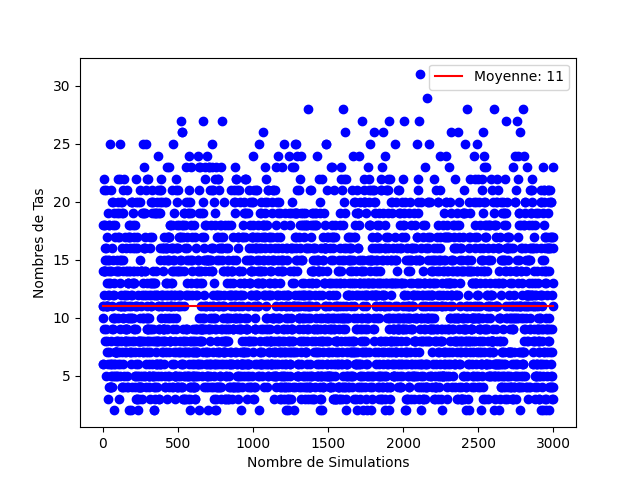
\includegraphics[scale=0.5]{stats_3000_32.png}
    \caption{Graphique représentant une simulation de 3000 parties avec 32 cartes}
\end{figure}

\begin{figure}[h]
    \centering
    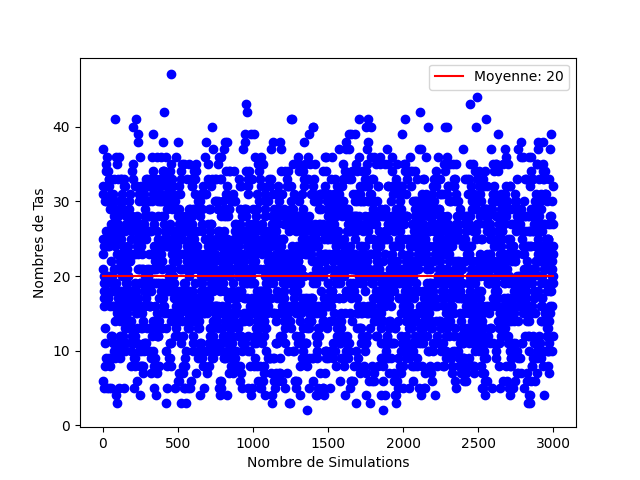
\includegraphics[scale=0.5]{stats_3000_52.png}
    \caption{Graphique représentant une simulation de 3000 parties avec 52 cartes}
\end{figure}


\subsection{Probabilité}
\noindent	\begin{minipage}{\textwidth}
	\begin{lstlisting}
	proba(nb_sim, nb_carte = 32)
	\end{lstlisting}	
	\end{minipage}

\emph{\textbf{conçue par : } Lucas Lesage} \vspace{2mm}\par

La fonction prend en argument 2 entiers : \textbf{nb\_sim} et \textbf{nb\_cartes} représentant le nombre de simulations ainsi que le nombre cartes désirées.  La fonction renvoie un dictionnaire contenant 32 ou 52 clés en fonction du nombre de carte voulu. \vspace{1mm}\par

L’objectif de cette fonction est de savoir exactement sur le nombre de simulation le nombre de fois où il y a eu 2 tas puis 3 et ainsi de suite jusqu’au nombre de carte. Ces données sont alors stockées dans un dictionnaire pour pouvoir accéder aux données facilement. \vspace{5mm}

\noindent	\begin{minipage}{\textwidth}
	\begin{lstlisting}
	graph_proba(nb_sim, nb_carte = 32)
	\end{lstlisting}	
	\end{minipage}

\emph{\textbf{conçue par : } Lucas Lesage} \vspace{2mm}\par

La fonction prend en argument 2 entiers : \textbf{nb\_sim} et \textbf{nb\_cartes} représentant le nombre de simulations ainsi que le nombre cartes désirées.  Elle ne renvoie rien mais affiche un graphique.

L’objectif de cette fonction est d’afficher la répartition des tas sur un nombre de simulations donnée. \par
La fonction est composée de 3 parties majeures. \par
Premièrement, cela va récupérer un dictionnaire généré par la fonction \texttt{proba}, puis va créer deux listes : \texttt{liste\_proba} et \texttt{liste\_probas}. La première est une liste de couples c’est-à-dire au format \texttt{[(clé, entier)]}. La deuxième quant à elle ne va contenir que les valeurs contenues dans le dictionnaire grâce à la fonction \texttt{dico\_to\_liste}, cette liste va permettre le calcule de la moyenne et de l’écart-type grâce à la bibliothèque numpy qui le permet. \par
Dans un deuxième temps la fonction va afficher les résultats sous la forme d’une fonction graphique. Pour cela, elle va utiliser la liste \texttt{liste\_proba} pour former des couples (x,y) grâce à la fonction zip. Par la suite, elle va tracer la fonction obtenue grâce au couple (x,y).\par

Et enfin dans un troisième temps, la fonction va regarder si le nombre de simulation est supérieur à 325. En effet, si le nombre de simulation est inférieur à 325 cela va lancer la génération d’une fonction représentant la densité de la loi Normal, obtenu grâce à la fonction \texttt{DensiteNormal} prenant en argument la moyenne et l’écart-type. La formule a été obtenu grâce à la formule mathématiques trouvable sur internet. Il devait y avoir aussi un histogramme représentant la loi normal associée mais malheureusement les résultats n’étaient pas satisfaisants d’un point de vue rendu. \par

Les problèmes obtenus sur la création de cette fonction ont été très nombreux comme la recherche autour de la génération d’une loi normal, mais aussi comment transformer un dictionnaire en tuples. Cela a nécessité énormément de recherches approfondies sur diverses plateformes montrant d’ailleurs l’immense possibilité derrière ces quelques modules que sont \texttt{matplotlib} et \texttt{numpy}.

\begin{figure}[h]
    \centering
    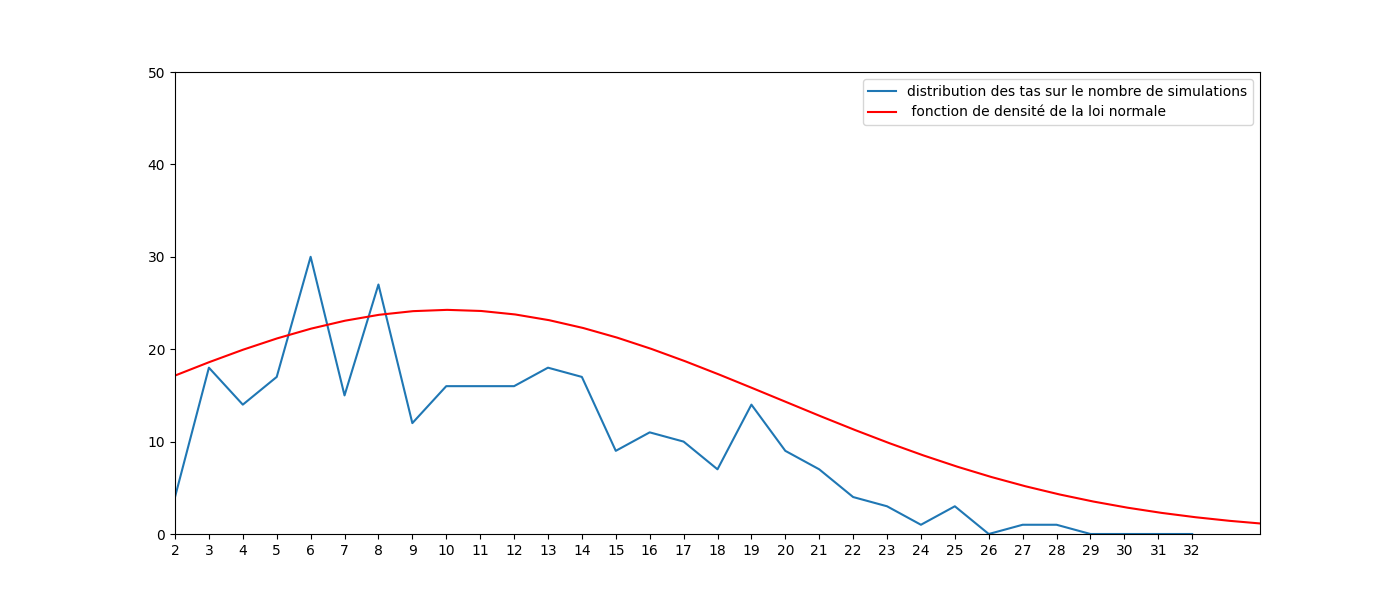
\includegraphics[scale=0.5]{proba_300_32.png}
    \caption{Graphique représentant une simulation de 300 parties avec 32 cartes}
\end{figure}

\begin{figure}[h]
    \centering
    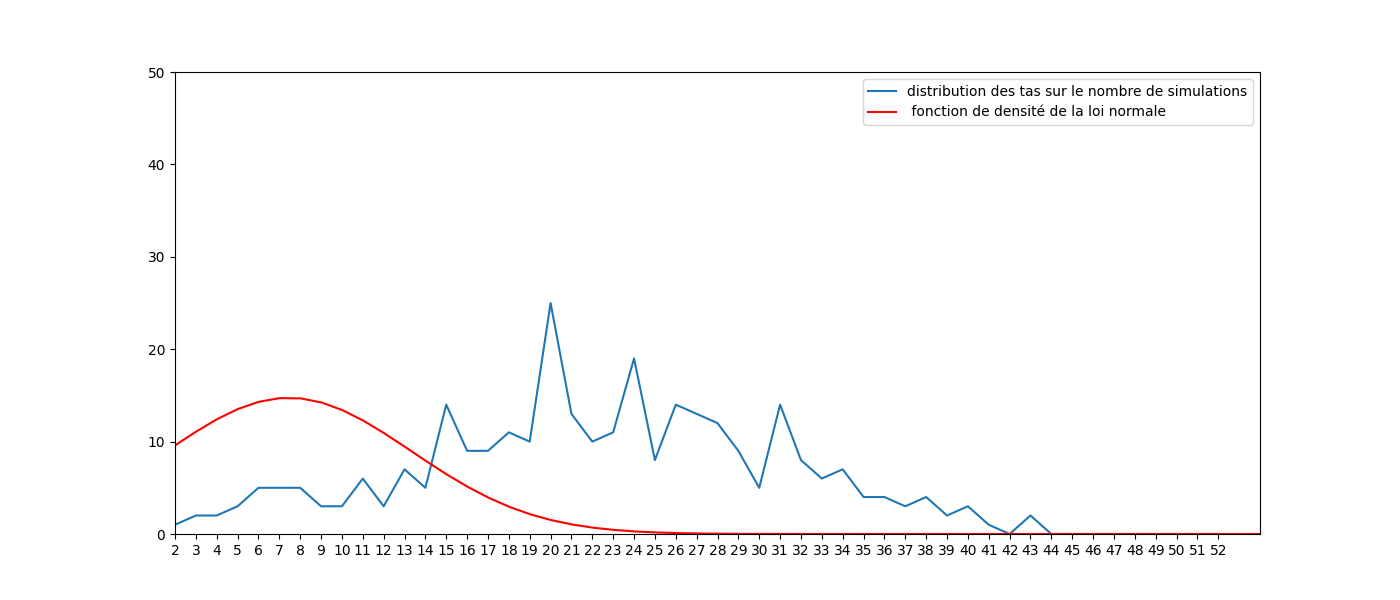
\includegraphics[scale=0.5]{proba_300_52.png}
    \caption{Graphique représentant une simulation de 300 parties avec 52 cartes}
\end{figure}

\vspace{5mm}

\subsection{Verifier Pioche}
\label{subsec : verif}
\noindent	\begin{minipage}{\textwidth}
	\begin{lstlisting}
	verifier_pioche(pioche, nb_cartes = 32) 
	\end{lstlisting}	
	\end{minipage}
	
\emph{\textbf{conçue par : } Lucas Lesage} \vspace{2mm}\par

La fonction prend en argument une liste pioche et un entier \textbf{nb\_cartes}. La fonction renvoie un booléen désignant si la pioche est complète et totalement juste.

L’objectif de cette fonction est de vérifier si un jeu de carte est correctement initialisé c’est-à-dire le bon nombre de carte et si elles y sont toutes. La Fonction va tout d’abord vérifier s’il y a le bon nombre de carte puis si la condition y est rentrée, elle va parcourir les cartes et vérifier les cartes une par une grâce à un compteur.


\newpage
\section*{Liste des fonctions présentées}
\addcontentsline{toc}{section}{Liste des fonctions présentées}

\subsection*{A - C}
\begin{description}
\item \texttt{afficher\_reussite}, section \ref{sec : principal}
\item \texttt{alliance}, section \ref{sec : principal}
\item \texttt{carte\_to\_chaine}, section \ref{sec : format}
\item \texttt{cree\_carte}, section \ref{sec : format}
\item \texttt{cree\_paquet\_cartes}, section \ref{sec : format}
\end{description}

\subsection*{E - I}
\begin{description}
\item \texttt{ecrire\_fichier\_reussite}, section \ref{sec : charg-sauv}
\item \texttt{graphique\_stats}, section \ref{sec : extensions}
\item \texttt{graph\_proba}, section \ref{sec : extensions}
\item \texttt{init\_pioche\_alea}, section \ref{sec : principal}
\item \texttt{init\_pioche\_alea}, section \ref{sec : charg-sauv}
\end{description}

\subsection*{L - P}
\begin{description}
\item \texttt{lance\_reussite}, section \ref{sec : modes_jeu}
\item \texttt{menu\_reussite}, section \ref{sec : menu}
\item \texttt{paquet\_to\_liste\_dico}, section \ref{sec : format}
\item \texttt{proba}, section \ref{sec : extensions}
\end{description}

\subsection*{R - V}
\begin{description}
\item \texttt{res\_multi\_simulation}, section \ref{sec : extensions}
\item \texttt{reussite\_mode\_auto}, section \ref{sec : modes_jeu}
\item \texttt{reussite\_mode\_manuel}, section \ref{sec : modes_jeu}
\item \texttt{saut\_si\_possible}, section \ref{sec : principal}
\item \texttt{statistiques\_nb\_tas}, section \ref{sec : extensions}
\item \texttt{une\_etape\_reussite}, section \ref{sec : principal}
\item \texttt{verifier\_pioche}, section \ref{sec : extensions}
\end{description}

\newpage
\section*{Bibliographie}
\addcontentsline{toc}{section}{Bibliographie}

\begin{itemize}
\item Daniel Diaz (15 juin 2021). \textit{7 façons de vérifier si un fichier ou un dossier existe en Python}. \\ \url{https://geekflare.com/fr/check-if-file-folder-exists-in-python/}
\item Documentation Matplotlib \\ \url{https://matplotlib.org/stable/users/index}
\end{itemize}


\end{document}